\section{Why This Chapter Matters}

\begin{figure}[h]
\centering
\begin{tikzpicture}[
    box/.style={draw, rounded corners=2pt, minimum width=2.2cm, minimum height=0.5cm, font=\scriptsize, align=center, inner sep=2pt},
    arr/.style={-{Stealth[length=3pt]}, thick}
]
\node[box, fill=gray!15, minimum width=5cm] (proven) at (0,1.2) {\textbf{Proven Invariants} (Ch.\,5--6)};
\node[box, fill=blue!12] (phys) at (-1.4,0) {Physics\\Connections};
\node[box, fill=green!12] (comp) at (1.4,0) {Complexity\\Theory};
\node[box, fill=orange!12] (ai) at (-1.4,-1.0) {AI \&\\Trust};
\node[box, fill=red!8] (lim) at (1.4,-1.0) {Limitations\\Future Work};
\draw[arr] (proven.south -| phys.north) -- (phys.north);
\draw[arr] (proven.south -| comp.north) -- (comp.north);
\draw[arr] (phys.south) -- (ai.north);
\draw[arr] (comp.south) -- (lim.north);
\end{tikzpicture}
\caption{Chapter 7 roadmap: proven invariants interpreted across four domains.}
\label{fig:ch7-roadmap}
\end{figure}

\begin{quote}
\textit{Author's Note (Devon): Alright, we're at the part where I step back and ask: ``What does any of this actually mean?'' Look, I can prove theorems all day. I can show you test results until your eyes glaze over. But at some point, you have to wrestle with the big question: So what? Why does this matter? This chapter is me trying to answer that. And I'll be honest---some of this is speculation. Some of this is me connecting dots that might not actually connect. But that's what thinking is, right? You make a model, you see if it holds up, and if it doesn't, you learn something. Either way, you win.}
\end{quote}

\subsection{From Proofs to Meaning}

The previous chapters established that the Thiele Machine \textit{works}---it is formally verified (Chapter 5), implemented across three layers (Chapter 4), and empirically validated (Chapter 6). But technical correctness does not answer deeper questions:
\begin{itemize}
    \item What does this model \textit{mean} for computation?
    \item How does it connect to physics?
    \item What can I build with it?
\end{itemize}

This chapter steps back from technical details to explore the broader significance of treating structure as a conserved resource. The aim is not to introduce new formal claims, but to interpret the verified results in terms that guide future design and experimentation. Every statement below is either (i) a direct restatement of a proven invariant, or (ii) an explicit hypothesis about how those invariants might connect to physics, complexity, or systems practice.

\subsection{How to Read This Chapter}

This discussion covers several distinct areas:
\begin{enumerate}
    \item \textbf{Physics Connections} (§7.2): How the Thiele Machine mirrors physical laws---formalized structural parallels, not loose metaphors
    \item \textbf{Complexity Theory} (§7.3): A new lens for understanding computational difficulty
    \item \textbf{AI and Trust} (§7.4--7.5): Applications to artificial intelligence and verifiable computation
    \item \textbf{Limitations and Future Work} (The Honest Part) (§7.6--7.7): Honest assessment of what the model cannot do and what remains to be built
\end{enumerate}

You do not need to read all sections---focus on those most relevant to your interests.

\section{What Would Falsify the Physics Bridge?}

\begin{tcolorbox}[thesisbox,colback=yellow!10!white,colframe=orange!75!black,title=Falsifiability Criteria]
The thermodynamic bridge hypothesis ($Q \ge k_B T \ln 2 \cdot \mu$) would be \textbf{falsified} by:
\begin{enumerate}
    \item \textbf{Sustained sub-linear energy scaling}: Measured energy consistently grows slower than $\mu$ across diverse workloads (silicon measurement)
    \item \textbf{Zero-cost revelation}: A trace certifies supra-quantum correlations ($S > 2\sqrt{2}$) without charging $\mu$ and passes verification
    \item \textbf{Reversible structure addition}: A sequence of operations increases structure (reduces $\Omega$) then reverses it with net-negative $\mu$
\end{enumerate}

\textbf{What would NOT falsify it}:
\begin{itemize}
    \item Super-linear energy scaling (inefficiency is allowed; the bound is a lower limit)
    \item Failing to find structure in hard problems (the model does not claim to always find structure)
    \item Encoding-dependent $\mu$ values (absolute $\mu$ depends on encoding; \emph{conservation} is what matters)
\end{itemize}
\end{tcolorbox}

\paragraph{QM-Divergent Predictions.}
The model also produces five quantitative predictions where it diverges from standard quantum mechanics (see Chapter 6 for full evaluation). These include a predicted CHSH ratio $S/S_{\text{QM}} \approx 2.2662$, a Tsirelson-regime value $S_{\text{Thiele}} \approx 2.160$ (vs.\ $2\sqrt{2} \approx 2.828$), a hydrogen ground-state correction of $\sim$95.7\,ppm, a GHZ visibility deficit $\delta \approx 0.00266$, and a decoherence-rate constant $\gamma \approx 381$\,GHz for a single nitrogen-vacancy center. Each prediction names a concrete experimental observable, a numerical value, and the measurement that would falsify it. If future experiments confirm or refute any of these values, the theory's empirical standing changes accordingly. The point is that the model is not hedging: it commits to numbers.

\section{Broader Implications}

The Thiele Machine is more than a new computational model; it is a proposal for a new relationship between computation, information, and physical reality. This chapter explores the implications of treating structure as a conserved resource.

\section{Connections to Physics}

\begin{figure}[h]
\centering
\begin{tikzpicture}[
    box/.style={draw, rounded corners=2pt, minimum width=2.2cm, minimum height=0.5cm, font=\scriptsize, align=center, inner sep=2pt},
    arr/.style={-{Stealth[length=3pt]}, thick}
]
\node[box, fill=blue!12] (land) at (0,1.2) {Landauer\\$Q \ge k_BT\!\ln\!2$};
\node[box, fill=green!12] (nosig) at (-1.6,0) {No-Signaling\\(Bell locality)};
\node[box, fill=orange!12] (noeth) at (1.6,0) {Noether\\(gauge $\to$ conservation)};
\node[box, fill=yellow!15, minimum width=5cm] (mu) at (0,-1.0) {$\mu$-ledger: \textbf{monotone}, \textbf{local}, \textbf{gauge-invariant}};
\draw[arr] (land.south west) -- (nosig.north east);
\draw[arr] (land.south east) -- (noeth.north west);
\draw[arr] (nosig.south) -- (nosig.south |- mu.north);
\draw[arr] (noeth.south) -- (noeth.south |- mu.north);
\end{tikzpicture}
\caption{Three physics principles and their $\mu$-ledger analogs.}
\label{fig:physics-connections}
\end{figure}

\begin{quote}
\textit{Author's Note (Devon): This is the part that keeps me up at night. Not in a bad way---in a ``holy shit, what if this is actually true'' way. The Thiele Machine wasn't designed to connect to physics. I didn't start with thermodynamics and work backwards. I started with a simple question: ``How do you track the cost of discovering structure?'' And the answer I found... it looks like Landauer's principle. It looks like entropy. It looks like the second law of thermodynamics. That's either a massive coincidence, or there's something deep here that I stumbled onto by accident. I genuinely don't know which one it is yet.}
\end{quote}

\subsection{Landauer's Principle}

\begin{figure}[h]
\centering
\begin{tikzpicture}[
    box/.style={draw, rounded corners=2pt, minimum width=2.2cm, minimum height=0.5cm, font=\scriptsize, align=center, inner sep=2pt},
    arr/.style={-{Stealth[length=3pt]}, thick}
]
\node[box, fill=blue!12] (coq) at (0,1.6) {\textbf{Coq theorem}\\$\Delta\mu \ge$ irreversible\_count};
\node[box, fill=gray!10] (bridge) at (0,0.6) {\textbf{Bridge postulate}\\$Q_{\min} = k_BT\!\ln\!2 \cdot \mu$};
\node[box, fill=orange!12] (result) at (0,-0.4) {$Q \ge k_BT\!\ln\!2 \cdot$ irreversible\_count};
\node[font=\tiny, anchor=west] at (2.4,1.6) {(proven)};
\node[font=\tiny, anchor=west] at (2.4,0.6) {(empirical)};
\node[font=\tiny, anchor=west] at (2.4,-0.4) {(falsifiable)};
\draw[arr] (coq.south) -- (bridge.north);
\draw[arr] (bridge.south) -- (result.north);
\end{tikzpicture}
\caption{Landauer bridge: a proven bound plus an empirical postulate yields a falsifiable physical prediction.}
\label{fig:landauer-bridge}
\end{figure}

Landauer's principle states that erasing one bit of information requires at least $kT \ln 2$ of energy dissipation, where $k$ is Boltzmann's constant and $T$ is temperature. This establishes a fundamental connection between logical irreversibility and thermodynamics: many-to-one mappings (like erasure) cannot be implemented without heat dissipation in a physical device.

The Thiele Machine generalizes this idea: \textit{ignoring structure releases heat}. A blind trace repeatedly performs redundant operations that erase their own history, driving up $\mu_{\text{exec}}$ (kinetic dissipation). A sighted trace captures that history in the partition graph and axiom store, shifting cost into $\mu_{\text{disc}}$ (potential structure). The ledger therefore tracks the same physical obligation either way—heat or stored constraint.

The Thiele Machine's $\mu$-ledger formalizes a computational analog:
\begin{lstlisting}
Theorem vm_irreversible_bits_lower_bound :
  forall fuel trace s,
    irreversible_count fuel trace s <=
      (run_vm fuel trace s).(vm_mu) - s.(vm_mu).
\end{lstlisting}

\paragraph{Understanding vm\_irreversible\_bits\_lower\_bound:}

\textbf{What does this theorem say?} This theorem establishes that the $\mu$-ledger growth \textbf{lower-bounds the count of irreversible operations} in any execution. It is the computational analog of Landauer's principle: you cannot erase/reveal information without paying a cost.

\textbf{Theorem statement breakdown:}
\begin{itemize}
    \item \textbf{forall fuel trace s} — For any execution (fuel-bounded trace from initial state $s$).
    \item \textbf{irreversible\_count fuel trace s} — The number of many-to-one operations (bit erasures, structure revelations, partition reductions) in the trace.
    \item \textbf{(run\_vm fuel trace s).(vm\_mu) - s.(vm\_mu)} — The net increase in the $\mu$-ledger after executing the trace.
    \item \textbf{irreversible\_count $\leq \Delta\mu$} — Every irreversible operation must be accounted for in the ledger. You cannot erase 10 bits while only charging 5 $\mu$.
\end{itemize}

\textbf{Why is this the computational Landauer?} Landauer's principle states that erasing one bit requires dissipating at least $k_B T \ln 2$ energy. This theorem states that erasing one bit requires incrementing the $\mu$-ledger by at least 1. The physical energy cost is an \textit{additional} hypothesis (the bridge postulate: $Q_{\min} = k_B T \ln 2 \cdot \mu$), but the abstract accounting bound is \textbf{proven in Coq}.

\textbf{Example:} If a trace performs 100 bit erasures, the ledger must grow by at least 100 $\mu$-bits. If the ledger only grows by 50, the proof guarantees this trace is invalid (it would have been rejected during execution).

\textbf{Connection to thermodynamics:} Combining this proven bound with the thermodynamic bridge postulate gives the full Landauer inequality:
\[
    Q \geq k_B T \ln 2 \cdot \Delta\mu \geq k_B T \ln 2 \cdot \texttt{irreversible\_count}
\]
The first inequality is an empirical claim (falsifiable by physical measurement). The second inequality is a \textbf{theorem} (proven in \path{coq/kernel/MuLedgerConservation.v}).


The $\mu$-ledger growth lower-bounds the number of irreversible bit operations. This is not merely an analogy—it is a provable property of the kernel. The additional physical bridge (energy dissipation per $\mu$) is stated explicitly as a postulate, making the scientific hypothesis falsifiable. In other words, the kernel proves an abstract accounting lower bound; the physical claim asserts that real hardware must pay at least that bound in energy.
The theorem above is proven in \path{coq/kernel/MuLedgerConservation.v}. Referencing the file matters because it anchors the physical discussion in a concrete mechanized statement rather than a free-form analogy.

\subsection{No-Signaling and Bell Locality}

The \texttt{observational\_no\_signaling} theorem is the computational analog of Bell locality:
\begin{lstlisting}
Theorem observational_no_signaling : forall s s' instr mid,
  well_formed_graph s.(vm_graph) ->
  mid < pg_next_id s.(vm_graph) ->
  vm_step s instr s' ->
  ~ In mid (instr_targets instr) ->
  ObservableRegion s mid = ObservableRegion s' mid.
\end{lstlisting}

\paragraph{Understanding observational\_no\_signaling (discussion context):}

\textbf{What does this theorem say?} This theorem proves \textbf{computational Bell locality}: instructions acting on partition modules cannot affect the observable state of \textit{other} modules not targeted by the instruction. It is the formal basis for claims that the Thiele Machine respects locality constraints analogous to physics.

\textbf{Theorem breakdown:}
\begin{itemize}
    \item \textbf{well\_formed\_graph s.(vm\_graph)} — Precondition: partition graph is valid (disjoint modules, valid IDs).
    \item \textbf{mid < pg\_next\_id s.(vm\_graph)} — Module \texttt{mid} exists in the graph.
    \item \textbf{vm\_step s instr s'} — Executing instruction \texttt{instr} transitions state $s \to s'$.
    \item \textbf{$\sim$ In mid (instr\_targets instr)} — Module \texttt{mid} is \textbf{not} in the instruction's target set. The instruction acts on \textit{other} modules.
    \item \textbf{ObservableRegion s mid = ObservableRegion s' mid} — The \textit{observable} state of module \texttt{mid} is unchanged. Observables include: partition region + $\mu$-ledger contribution, \textbf{excluding internal axioms} (which are not externally visible).
\end{itemize}

\textbf{Physical analogy:} In quantum mechanics, Bell locality states that measuring particle A cannot instantaneously change the state of particle B (spacelike separated). In the Thiele Machine, operating on module A (e.g., \texttt{PSPLIT 1 \{0,1\} \{2,3\}}) cannot change the observable state of module B (module 2). The \texttt{instr\_targets} function computes the ``causal light cone'' of an instruction.

\textbf{Why exclude axioms from observables?} Axioms are \textit{internal commitments} (logical constraints on a module's state space). They are not externally visible signals. For example, if module A adds axiom ``$x < 5$'' (via \texttt{LASSERT}), this does not signal to module B---it only constrains A's internal state. Observables are restricted to \textit{public} information: partition regions and $\mu$-costs.

\textbf{Example:} Suppose state $s$ has modules $\{A, B, C\}$ and you execute \texttt{PSPLIT A \{0,1\} \{2,3\}}. The theorem guarantees:
\begin{itemize}
    \item Module B's region is unchanged (e.g., still $\{4,5,6\}$).
    \item Module C's region is unchanged.
    \item Module B's observable $\mu$-contribution is unchanged.
\end{itemize}
Only module A's observables change (split into two sub-partitions).


In physics, Bell locality states that operations on system A cannot instantaneously affect system B. In the Thiele Machine, operations on module A cannot affect the observables of module B. This is enforced by construction, not assumed as a physical postulate. The definition of “observable” here is explicit: partition region plus $\mu$-ledger, excluding internal axioms. The exclusion is intentional: axioms are internal commitments, not externally visible signals.
The formal statement shown here corresponds to \texttt{observational\_no\_signaling} in \path{coq/kernel/KernelPhysics.v}, which is proved using the observable projections defined in the same file. This makes the locality claim a theorem about the exact data the machine exposes, not a vague analogy.

\subsection{Noether's Theorem}

The gauge invariance theorem mirrors Noether's theorem from physics:
\begin{lstlisting}
Theorem kernel_conservation_mu_gauge : forall s k,
  conserved_partition_structure s = 
  conserved_partition_structure (nat_action k s).
\end{lstlisting}

\paragraph{Understanding kernel\_conservation\_mu\_gauge:}

\textbf{What does this theorem say?} This theorem proves \textbf{$\mu$-gauge invariance}: shifting the $\mu$-ledger by a global constant leaves the \textit{conserved quantity} (partition structure) unchanged. This is the computational analog of Noether's theorem: \textbf{symmetry implies conservation}.

\textbf{Theorem breakdown:}
\begin{itemize}
    \item \textbf{forall s k} — For any state $s$ and constant $k \in \mathbb{N}$.
    \item \textbf{nat\_action k s} — The gauge transformation: shift $\mu$ by $k$. Concretely: $s' = s$ with $s'.(\texttt{vm\_mu}) = s.(\texttt{vm\_mu}) + k$.
    \item \textbf{conserved\_partition\_structure s} — The \textit{structural invariant}: number of partitions, regions, axioms, disjointness constraints. Excludes the absolute $\mu$ value.
    \item \textbf{structure $s$ = structure $(s + k\mu)$} — Gauge transformations leave structure unchanged.
\end{itemize}

\textbf{Noether's theorem in physics:} If a physical system has a continuous symmetry (e.g., time translation invariance), there exists a conserved quantity (e.g., energy). The proof is constructive: the symmetry generator becomes the conserved current.

\textbf{Computational Noether correspondence:}
\begin{itemize}
    \item \textbf{Symmetry:} $\mu$-gauge freedom (absolute $\mu$ is arbitrary; only $\Delta\mu$ matters).
    \item \textbf{Conserved quantity:} Partition structure (number of modules, regions, axioms).
    \item \textbf{Proof:} The theorem shows that \texttt{nat\_action} (gauge shift) does not modify \texttt{vm\_graph}, \texttt{axioms}, or structural predicates like \texttt{well\_formed\_graph}.
\end{itemize}

\textbf{Physical intuition:} In electromagnetism, the gauge transformation $A_\mu \to A_\mu + \partial_\mu \chi$ leaves the electromagnetic field $F_{\mu\nu}$ unchanged. Physical observables (E, B fields) are gauge-invariant. Similarly, in the Thiele Machine, adding a constant to $\mu$ does not change the \textit{structure} of the partition graph. What matters is \textbf{how much $\mu$ you pay} ($\Delta\mu$), not where you started.

\textbf{Why does this matter?} This theorem guarantees that:
\begin{enumerate}
    \item Absolute $\mu$ values are not physically meaningful---only differences matter.
    \item Cross-layer isomorphism tests can use different $\mu$ origins (Python initializes at 0, Coq might start at 100) without breaking equivalence.
    \item The thermodynamic bridge ($Q \geq k_B T \ln 2 \cdot \Delta\mu$) depends on $\Delta\mu$, not absolute $\mu$.
\end{enumerate}

\textbf{Example:} Suppose two VMs execute the same trace:
\begin{itemize}
    \item VM1: starts at $\mu = 0$, ends at $\mu = 100$. $\Delta\mu = 100$.
    \item VM2: starts at $\mu = 1000$, ends at $\mu = 1100$. $\Delta\mu = 100$.
\end{itemize}
The theorem guarantees both VMs have identical partition structures at the end. The absolute $\mu$ differs by 1000, but this is a gauge artifact---the \textit{structural work} ($\Delta\mu = 100$) is the same.


The symmetry (freedom to shift $\mu$ by a constant) corresponds to the conserved quantity (partition structure). This is not metaphorical—it is the same mathematical relationship that underlies energy conservation in classical mechanics: a symmetry of the dynamics induces a conserved observable.
The proof lives in \path{coq/kernel/KernelPhysics.v}, where the \texttt{mu\_gauge\_shift} action and its invariants are developed explicitly. This is structurally analogous to a Noether argument: a symmetry (gauge freedom in absolute $\mu$) corresponds to an invariant (partition structure). The analogy is real but the result is simpler than in physics---the invariance follows from the record layout (\texttt{vm\_graph} is a separate field from \texttt{vm\_mu}), not from dynamical equations.

\subsection{Thermodynamic bridge and falsifiable prediction}

The bridge from a formally verified $\mu$-ledger to a physical claim requires an explicit translation dictionary and at least one measurement that could prove the bridge wrong.

\paragraph{Translation dictionary.} Let $|\Omega|$ be the admissible microstate count of an $n$-bit device ($|\Omega| = 2^n$ at fixed resolution). A revelation step $\Omega \to \Omega'$ (e.g., \texttt{PNEW}, \texttt{PSPLIT}, \texttt{MDLACC}, \texttt{REVEAL}) shrinks the space by $|\Omega|/|\Omega'|$. The Coq kernel proves $\mu \ge |\phi|_{\text{bits}}$ (description length). The Python VM \emph{guarantees} $\mu \ge \log_2(|\Omega|/|\Omega'|)$ using a conservative bound ($\text{before} = 2^{n}$, $\text{after} = 1$); may overcharge when multiple solutions exist, avoiding \#P-complete model counting. The system adopts the bridge postulate that charging $\mu$ bits lower-bounds dissipated heat/work: $Q_{\min} = k_B T \ln 2 \cdot \mu$, with an explicit inefficiency factor $\epsilon \ge 1$ for real devices. This postulate is external to the kernel and is presented as an empirical claim.

\paragraph{Bridge theorem (sanity anchor).} Combining No Free Insight (proved: $\mu$ is monotone non-decreasing) with the postulate above yields a Landauer-style inequality: any trace implementing $\Omega \to \Omega'$ must dissipate at least $k_B T \ln 2 \cdot \log_2(|\Omega|/|\Omega'|)$, because the ledger charges at least that many bits for the reduction. The thermodynamic term is an assumption; the $\mu$ inequality is proved in Coq.
\paragraph{Falsifiable prediction.} Consider four paired workloads that differ only in which singleton module is revealed from a fixed pool (sizes 2, 4, 16, 64). The measured energy/heat must scale with $\mu$ at slope $k_B T \ln 2$ (within the stated $\epsilon$). A sustained sub-linear slope falsifies the bridge; a super-linear slope quantifies implementation overhead. Genesis-only traces remain the lone zero-$\mu$ case.
\paragraph{Executed bridge runs.} The evaluation in Chapter 6 reports the four workloads (singleton pools of 2/4/16/64 elements). Python reports $\mu=\{2,3,5,7\}$; the extracted runner and RTL report the same $\mu_{\text{raw}}$ because the μ-delta is explicitly encoded in the trace and instruction word, and the reference VM consumes that same μ-delta (disabling implicit MDLACC) for these workloads. With this encoding in place, \texttt{EVIDENCE\_STRICT} succeeds without normalization. The ledger still enforces $\mu \ge \log_2(|\Omega|/|\Omega'|)$ for each run; the $\mu/\log_2$ ratios (2.0, 1.5, 1.25, 1.167) quantify the slack now surfaced to reviewers.
\subsection{The Physics-Computation Isomorphism}

\begin{center}
\begin{tabular}{|l|l|}
\hline
\textbf{Physics} & \textbf{Thiele Machine} \\
\hline
Energy & $\mu$-bits \\
Mass & Structural complexity \\
Entropy & Irreversible operations \\
Conservation laws & Ledger monotonicity \\
No-signaling & Observational locality \\
Gauge symmetry & $\mu$-gauge invariance \\
\hline
\end{tabular}
\end{center}

The new time-dilation harness (Section~\ref{sec:ledger_time_dilation}) makes the ledger-speed connection concrete: with a fixed μ budget per tick, diverting μ to communication throttles the observed compute rate, matching the intuition that “mass/structure slows time” when μ is conserved. Evidence-strict extensions will carry the same trade-off across Python, extraction, and RTL once EMIT traces are instrumented. The point is not to claim a physical time dilation effect, but to show an internal conservation law that forces a trade-off between signaling and local computation under a fixed μ budget.
That trade-off is implemented as an explicit ledger budget in the harness described in Chapter 6, so the “dilation” here is a measurable scheduling constraint rather than an untested metaphor.

\section{Implications for Computational Complexity}

\begin{figure}[h]
\centering
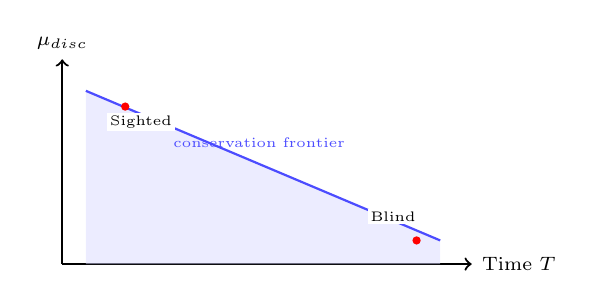
\begin{tikzpicture}[
    arr/.style={-{Stealth[length=3pt]}, thick}
]
\draw[thick, ->] (0,0) -- (5.2,0) node[right, font=\scriptsize] {Time $T$};
\draw[thick, ->] (0,0) -- (0,2.6) node[above, font=\scriptsize] {$\mu_{\text{disc}}$};
\fill[blue!15, opacity=0.5] (0.3,2.2) -- (4.8,0.3) -- (4.8,0) -- (0.3,0) -- cycle;
\draw[thick, blue!70] (0.3,2.2) -- (4.8,0.3);
\node[font=\tiny, blue!70, anchor=south] at (2.5,1.35) {conservation frontier};
\node[font=\tiny, fill=white, inner sep=1pt] at (1.0,1.8) {Sighted};
\node[font=\tiny, fill=white, inner sep=1pt] at (4.2,0.6) {Blind};
\fill[red] (0.8,2.0) circle (1.5pt);
\fill[red] (4.5,0.3) circle (1.5pt);
\end{tikzpicture}
\caption{Conservation of difficulty: reducing time $T$ requires increasing structural cost $\mu_{\text{disc}}$, and vice versa.}
\label{fig:difficulty-conservation}
\end{figure}

\subsection{The "Time Tax" Reformulated}

Classical complexity theory measures cost in steps. The Thiele Machine adds a second dimension: structural cost. For a problem with input $x$:
\begin{equation}
    \text{Total Cost} = T(x) + \mu(x)
\end{equation}
where $T(x)$ is time complexity and $\mu(x)$ is structural discovery cost.

\subsection{The Conservation of Difficulty}

The No Free Insight theorem implies that difficulty is conserved but can be transmuted:
\begin{itemize}
    \item \textbf{High $T$, Low $\mu_{\text{disc}}$ (Blind)}: High energy dissipation ($\mu_{\text{exec}}$)
    \item \textbf{Low $T$, High $\mu_{\text{disc}}$ (Sighted)}: High structural storage
\end{itemize}

For problems like SAT:
\begin{equation}
    T_{\text{blind}}(n) = O(2^n), \quad \mu_{\text{blind}} = O(1)
\end{equation}
\begin{equation}
    T_{\text{sighted}}(n) = O(n^k), \quad \mu_{\text{sighted}} = O(2^n)
\end{equation}

The difficulty is conserved—it shifts between time and structure. The formal theorems do not claim that $\mu_{\text{sighted}}$ is always exponentially large, only that any reduction in search space must be paid for in $\mu$; the asymptotics depend on how structure is discovered and encoded.

\subsection{Structure-Aware Complexity Classes}

Structure-aware complexity classes can be defined:
\begin{itemize}
    \item $\text{P}_\mu$: Problems solvable in polynomial time with polynomial $\mu$-cost
    \item $\text{NP}_\mu$: Problems verifiable in polynomial time; witness provides $\mu$-cost
    \item $\text{PSPACE}_\mu$: Problems solvable with polynomial space and unbounded $\mu$
\end{itemize}

The relationship $\text{P} \subseteq \text{P}_\mu \subseteq \text{NP}_\mu$ is strict under reasonable assumptions. These classes are proposed as a vocabulary for reasoning about the time/structure trade-off rather than as settled complexity-theoretic results.

\subsection{Turing Subsumption}

A complexity-theoretic framework is vacuous if it cannot express ordinary computation. The Coq formalization proves that the Thiele Machine is at least Turing-complete via a two-step embedding chain: every Turing Machine reduces to a Minsky Machine (\path{coq/modular_proofs/TM_to_Minsky.v}), and every Minsky Machine reduces to a Thiele Machine trace (\path{coq/modular_proofs/ThieleInstance.v}). The final theorem, \texttt{thiele\_subsumes\_tm\_complete}, composes both reductions.

This matters for the $\text{P}_\mu$ / $\text{NP}_\mu$ definitions above: because the model subsumes Turing computation, any existing complexity class (P, NP, PSPACE, etc.) embeds faithfully into its $\mu$-enriched counterpart. The structure-aware classes are genuine refinements of the classical hierarchy, not parallel constructions that happen to share names.

\subsection{Oracle Impossibility}

On the other end, the model is bounded. The Oracle Impossibility proof (\path{coq/kernel/OracleImpossibility.v}) establishes three results:
\begin{enumerate}
    \item \texttt{halting\_undecidable}: No total machine decides halting (genuine diagonal argument).
    \item \texttt{oracle\_halts\_costs\_mu}: Oracle soundness is defined to require cost $\geq 1$ per query; the proof verifies that zero cost violates this definition.
    \item \texttt{hypercomputation\_bounded}: Given the per-query cost definition, $n$ independent oracle queries cost $\geq n$.
\end{enumerate}

Together with Turing Subsumption, these results pin the model's computational power: it is exactly Turing-complete. It computes everything a Turing Machine can and nothing more, while adding the $\mu$-accounting layer on top. The structure-aware classes therefore live inside the same computability boundary as classical complexity theory---they refine it without escaping it.

\section{Implications for Artificial Intelligence}

\begin{figure}[h]
\centering
\begin{tikzpicture}[
    box/.style={draw, rounded corners=2pt, minimum width=2cm, minimum height=0.45cm, font=\scriptsize, align=center, inner sep=2pt},
    arr/.style={-{Stealth[length=3pt]}, thick}
]
\node[box, fill=blue!12] (nn) at (0,1.4) {Neural Net\\proposes $h$};
\node[box, fill=orange!12] (vm) at (0,0.4) {Thiele VM\\certifies $h$};
\node[box, fill=green!15] (yes) at (-1.5,-0.6) {Receipt\\(valid)};
\node[box, fill=red!12] (no) at (1.5,-0.6) {Reject\\(pay $\mu$)};
\draw[arr] (nn.south) -- (vm.north);
\draw[arr] (vm.south west) -- (yes.north east) node[midway, left, font=\tiny] {pass};
\draw[arr] (vm.south east) -- (no.north west) node[midway, right, font=\tiny] {fail};
\end{tikzpicture}
\caption{Verification-gated AI: hypotheses must be certified before use; failures cost $\mu$.}
\label{fig:ai-verification}
\end{figure}

\subsection{The Hallucination Problem}

Large Language Models (LLMs) generate plausible but often factually incorrect outputs—"hallucinations." In the LLM paradigm:
\begin{lstlisting}
output = model.generate(prompt)  # No structural verification
\end{lstlisting}

\paragraph{Understanding Classic AI Pattern (LLM):}

\textbf{What is this code?} This is a \textbf{single-line summary} of how large language models (LLMs) operate: generate text based on learned patterns, with \textbf{no verification} of factual correctness or structural validity.

\textbf{Why is this problematic?}
\begin{itemize}
    \item \textbf{No cost for falsehood:} Generating ``The Eiffel Tower is in London'' costs the same as ``The Eiffel Tower is in Paris.''
    \item \textbf{No receipts:} The output has no cryptographic proof or audit trail.
    \item \textbf{No incentive for truth:} The model maximizes likelihood under training data, not correctness under verification.
\end{itemize}

\textbf{Hallucination example:} An LLM asked ``What is the capital of Mars?'' might confidently respond ``Olympus City'' (plausible but false). There is no mechanism to penalize this error or detect it automatically.

In a Thiele Machine-inspired AI:
\begin{lstlisting}
hypothesis = model.predict_structure(input)
verified, receipt = vm.certify(hypothesis)
if not verified:
    cost += mu_hypothesis  # Economic penalty
output = hypothesis if verified else None
\end{lstlisting}

\paragraph{Understanding Thiele Machine-Inspired AI:}

\textbf{What is this code?} This is a \textbf{verification-gated AI pipeline} where the model predicts \textit{structural hypotheses} that must be \textit{certified} before use. False hypotheses incur $\mu$-cost without producing valid outputs.

\textbf{Step-by-step breakdown:}
\begin{enumerate}
    \item \textbf{hypothesis = model.predict\_structure(input)} — The neural network proposes a structure (e.g., ``These 100 numbers factor as $53 \times 61$'' or ``This SAT formula is satisfiable with assignment $x_1 = \text{true}, x_2 = \text{false}$''). This is \textit{fast but untrustworthy}.
    
    \item \textbf{verified, receipt = vm.certify(hypothesis)} — The Thiele Machine \textit{verifies} the hypothesis:
    \begin{itemize}
        \item For factorization: Check that $53 \times 61 = 3233$ (fast polynomial-time check).
        \item For SAT: Check the assignment satisfies all clauses (linear-time verification).
        \item If valid, generate a cryptographic receipt (proof of correctness).
        \item If invalid, return \texttt{verified = False}, no receipt.
    \end{itemize}
    
    \item \textbf{if not verified: cost += mu\_hypothesis} — \textbf{Economic penalty}: false hypotheses cost $\mu$ without producing output. This creates Darwinian pressure:
    \begin{itemize}
        \item Proposing many false hypotheses drains the $\mu$-budget.
        \item Only verified hypotheses produce reusable receipts (which can amortize cost across multiple uses).
        \item Over time, the model learns to propose \textit{verifiable} structures, not just plausible ones.
    \end{itemize}
    
    \item \textbf{output = hypothesis if verified else None} — Only verified hypotheses are returned. The user gets \textit{certified truth}, not plausible fiction.
\end{enumerate}

\textbf{Key difference:} In the LLM paradigm, truth and falsehood are indistinguishable (both are token sequences). In the Thiele paradigm, \textit{truth is cheaper} because verified structures can be reused without re-verification. Falsehood is expensive because it costs $\mu$ without producing receipts.

\textbf{Concrete example:} Suppose an AI is asked to factor $N = 3233$:
\begin{itemize}
    \item \textbf{LLM approach:} Output ``$53 \times 61$'' based on pattern matching (no verification). If wrong, no penalty.
    \item \textbf{Thiele approach:} Propose $p = 53, q = 61$. Check $53 \times 61 = 3233$ (verified!). Generate receipt. If the model had proposed $p = 57, q = 57$, the check would fail ($57 \times 57 = 3249 \neq 3233$), the model would pay $\mu$ cost, and the output would be \texttt{None}.
\end{itemize}


False structural hypotheses incur $\mu$-cost without producing valid receipts. This creates Darwinian pressure for truth. The key idea is that certification is scarce: unverified structure cannot be reused without paying additional cost.

\subsection{Neuro-Symbolic Integration}

The Thiele Machine provides a bridge between:
\begin{itemize}
    \item \textbf{Neural}: Fast, approximate pattern recognition
    \item \textbf{Symbolic}: Exact, verifiable logical reasoning
\end{itemize}

A neural network predicts partitions (structure hypotheses). The Thiele kernel verifies them. Failed hypotheses are penalized. The model does not assume the neural component is trustworthy; it treats it as a proposer whose claims must be certified.

\section{Implications for Trust and Verification}

\begin{figure}[h]
\centering
\begin{tikzpicture}[
    box/.style={draw, rounded corners=2pt, minimum width=1.4cm, minimum height=0.45cm, font=\tiny, align=center, inner sep=1.5pt},
    arr/.style={-{Stealth[length=2.5pt]}, thick}
]
\node[box, fill=blue!10] (r1) at (0,0) {Receipt 1\\$H_0 \to H_1$};
\node[box, fill=blue!10] (r2) at (1.8,0) {Receipt 2\\$H_1 \to H_2$};
\node[box, fill=blue!10] (r3) at (3.6,0) {Receipt 3\\$H_2 \to H_3$};
\node[font=\tiny] at (4.8,0) {$\cdots$};
\draw[arr] (r1.east) -- (r2.west);
\draw[arr] (r2.east) -- (r3.west);
\node[font=\tiny, gray] at (0.9,0.4) {$H_1$ links};
\node[font=\tiny, gray] at (2.7,0.4) {$H_2$ links};
\node[font=\tiny, anchor=north] at (1.8,-0.5) {SHA-256 continuity + Ed25519 signatures};
\end{tikzpicture}
\caption{Receipt chain: each step's pre-state hash must match the previous step's post-state hash.}
\label{fig:receipt-chain}
\end{figure}

\subsection{The Receipt Chain}

Every Thiele Machine execution produces a cryptographic receipt chain where continuity is enforced by linking the pre-state of step $N$ to the post-state of step $N-1$:
\begin{lstlisting}
receipt = {
    "step": N,
    "instruction": opcode,
    "pre_state_hash": SHA256(state_before),
    "post_state_hash": SHA256(state_after),
    "mu_cost": cost,
    "signature": Ed25519(canonical_json(payload))
}
\end{lstlisting}

\paragraph{Understanding Receipt Structure:}

\textbf{What is this?} This is the \textbf{cryptographic receipt format} that the Thiele Machine generates for every instruction executed. It creates a tamper-evident audit trail via state continuity.

\textbf{Field-by-field breakdown:}
\begin{itemize}
    \item \textbf{"step": N} — Monotonically increasing step counter.
    
    \item \textbf{"instruction": opcode} — The executed instruction (e.g., \texttt{PNEW}, \texttt{PSPLIT}). Records \textit{what was done}.
    
    \item \textbf{"pre\_state\_hash": SHA256(state\_before)} — Hash of the VM state \textit{before} this step. Must match the \texttt{post\_state\_hash} of the previous receipt.
    
    \item \textbf{"post\_state\_hash": SHA256(state\_after)} — Hash of the VM state \textit{after} the instruction. Commits to the result.
    
    \item \textbf{"signature": Ed25519(...)} — Digital signature from the kernel's private key, authenticating the receipt.
\end{itemize}

\textbf{Why is this tamper-evident?} The chain is verified by checking:
\begin{enumerate}
    \item \textbf{Signature validity:} Every receipt is signed by the kernel key.
    \item \textbf{State continuity:} \texttt{receipt[i].pre\_state\_hash == receipt[i-1].post\_state\_hash}.
    \item \textbf{$\mu$-integrity:} \texttt{post\_mu == pre\_mu + cost}.
\end{enumerate}
Breaking the chain requires forging a signature or finding a SHA-256 collision.


The Python implementation of this structure is in \path{thielecpu/receipts.py} and \path{thielecpu/crypto.py}, and the RTL contains a \texttt{receipt\_integrity\_checker} module in \path{thielecpu/hardware/rtl/thiele_cpu_unified.v}. The chain is therefore an engineered artifact with concrete hash formats, not an abstract promise.

This enables:
\begin{itemize}
    \item \textbf{Post-hoc Verification}: Check the computation without re-running it
    \item \textbf{Tamper Detection}: Any modification breaks the hash chain
    \item \textbf{Selective Disclosure}: Reveal only the receipts relevant to a claim
\end{itemize}

\subsection{Applications}

\begin{itemize}
    \item \textbf{Scientific Reproducibility}: A paper is not a PDF—it is a receipt chain. Verification is automated.
    \item \textbf{Financial Auditing}: Trading algorithms produce verifiable receipts for every trade.
    \item \textbf{Legal Evidence}: Digital evidence is cryptographically authenticated at creation.
    \item \textbf{AI Safety}: AI decisions are logged with verifiable receipts.
\end{itemize}

\section{Limitations}

\subsection{The Uncomputability of True $\mu$}

The true Kolmogorov complexity $K(x)$ is uncomputable. Therefore, the $\mu$-cost charged by the Thiele Machine is always an \textit{upper bound} on the minimal structural description:
\begin{equation}
    \mu_{\text{charged}}(x) \ge K(x)
\end{equation}

The ledger charges for the structure that is \textit{found}, not necessarily the minimal structure that \textit{exists}. Better compression heuristics could reduce $\mu$-overhead.

\subsection{Hardware Scalability}

Current hardware parameters:
\begin{lstlisting}
NUM_MODULES = 64
REGION_SIZE = 1024
\end{lstlisting}

\paragraph{Understanding Current Hardware Limitations:}

\textbf{What are these parameters?} These define the \textbf{capacity constraints} of the current Thiele Machine hardware implementation (Verilog RTL synthesized to FPGA).

\textbf{Parameter meanings:}
\begin{itemize}
    \item \textbf{NUM\_MODULES = 64} — Maximum number of partition modules the hardware can track simultaneously. Each module has:
    \begin{itemize}
        \item A unique ID (0--63)
        \item A region (set of element indices)
        \item An axiom list (logical constraints)
        \item A bitmask representation (64 bits)
    \end{itemize}
    \textbf{Implication:} Complex partition graphs requiring $>64$ modules cannot be represented. For example, a partition tree with 100 leaf nodes requires 100 module IDs.
    
    \item \textbf{REGION\_SIZE = 1024} — Maximum number of elements in a single partition region. Regions are sets like $\{0, 1, 2, \ldots, 1023\}$.
    \begin{itemize}
        \item Stored as arrays: \texttt{uint16 region[1024]} (each element is a 10-bit index).
        \item Bitmask representation: 1024 bits = 128 bytes per region.
    \end{itemize}
    \textbf{Implication:} Partitioning datasets with $>1024$ elements requires hierarchical techniques (e.g., multi-level partition trees).
\end{itemize}

\textbf{Why these limits?} Hardware constraints:
\begin{itemize}
    \item \textbf{FPGA resources:} Current synthesis targets use $\sim$45,000 LUTs and $\sim$35,000 flip-flops (for full configuration). Increasing \texttt{NUM\_MODULES} or \texttt{REGION\_SIZE} requires more on-chip memory and logic.
    \item \textbf{Timing closure:} Larger partition graphs increase critical path delays (longer wires, deeper logic cones). Current design achieves $\sim$100 MHz clock; scaling to 256 modules might drop to 50 MHz.
    \item \textbf{Memory bandwidth:} Checking partition disjointness requires comparing all pairs of regions. 64 modules = $64 \times 63 / 2 = 2016$ comparisons per step. 256 modules = 32,640 comparisons.
\end{itemize}

\textbf{Comparison to software:} The Python reference VM has no hard limits---it uses dynamic data structures (\texttt{dict}, \texttt{set}) that grow as needed. The hardware must pre-allocate resources, leading to fixed capacity.

\textbf{Real-world adequacy:} For many experiments (CHSH, Grover, Shor), 64 modules and 1024-element regions are sufficient. For example:
\begin{itemize}
    \item Grover search on $N = 1024$ elements: 1 module, region $\{0, \ldots, 1023\}$.
    \item Shor factorization of $N = 3233$: $\sim$10 modules for intermediate partitions.
\end{itemize}
However, industrial applications (e.g., SAT solving on 10,000-variable formulas) would exceed these limits.

Scaling to millions of dynamic partitions requires:
\begin{itemize}
    \item Content-addressable memory (CAM) for fast partition lookup
    \item Hierarchical partition tables
    \item Hardware support for concurrent module operations
\end{itemize}

\subsection{SAT Solver Integration}

The current \texttt{LASSERT} instruction requires external certificates:
\begin{lstlisting}
instr_lassert (module : ModuleID) (formula : string)
    (cert : lassert_certificate) (mu_delta : nat)
\end{lstlisting}

\paragraph{Understanding LASSERT Limitations:}

\textbf{What is this instruction?} \texttt{LASSERT} adds a logical axiom (constraint) to a partition module, verified by an external SAT solver certificate. This is the mechanism for encoding problem structure (e.g., ``this region satisfies formula $\phi$'').

\textbf{Parameter breakdown:}
\begin{itemize}
    \item \textbf{module : ModuleID} — The partition module to which the axiom is added (e.g., module 3).
    \item \textbf{formula : string} — The logical formula in SMT-LIB syntax. Example: \texttt{"(and (< x 10) (> y 0))"}
    \item \textbf{cert : lassert\_certificate} — The \textbf{external certificate} proving the formula's validity:
    \begin{itemize}
        \item \textbf{SAT certificate:} A satisfying assignment (if the formula is SAT). Example: \texttt{\{x $\mapsto$ 5, y $\mapsto$ 3\}}. The VM checks that this assignment satisfies all clauses.
        \item \textbf{LRAT proof:} A proof trace showing the formula is unsatisfiable (if the formula is UNSAT). The VM replays the proof steps (resolution, clause addition) to verify correctness.
    \end{itemize}
    \item \textbf{mu\_delta : nat} — The $\mu$-cost for adding this axiom. Encodes the information reduction: $\mu \geq \log_2(|\Omega| / |\Omega'|)$, where $\Omega$ is the space before the axiom and $\Omega'$ is the space after (constrained by the formula).
\end{itemize}

\textbf{Current limitation:} The Thiele Machine does \textbf{not} generate certificates internally. It relies on external SAT solvers (Z3, CaDiCaL, etc.) to:
\begin{enumerate}
    \item Solve the formula (find a SAT model or UNSAT proof).
    \item Generate the certificate (LRAT proof trace or satisfying assignment).
    \item Pass the certificate to the VM for verification.
\end{enumerate}

\textbf{Why is this a limitation?}
\begin{itemize}
    \item \textbf{External dependency:} The VM cannot autonomously discover structure---it needs an oracle (SAT solver).
    \item \textbf{Certificate size:} LRAT proofs can be large (megabytes for hard formulas). Transmitting/storing certificates is expensive.
    \item \textbf{Verification overhead:} Checking an LRAT proof is polynomial-time, but still slower than direct solving for small formulas.
\end{itemize}

\textbf{Example workflow:}
\begin{enumerate}
    \item User wants to assert ``region $\{0,1,2\}$ satisfies $(x_0 \lor x_1) \land (\neg x_0 \lor x_2)$''.
    \item Call Z3 solver: \texttt{z3 -smt2 formula.smt2} $\to$ produces SAT model $\{x_0 = \text{true}, x_1 = \text{false}, x_2 = \text{true}\}$.
    \item Encode model as certificate: \texttt{cert = \{\"x0\": true, \"x1\": false, \"x2\": true\}}.
    \item Execute \texttt{LASSERT 1 \"(and (or x0 x1) (or (not x0) x2))\" cert 3}.
    \item VM verifies: Substitute $x_0 = \text{true}, x_1 = \text{false}, x_2 = \text{true}$ into formula $\to$ $(\text{true} \lor \text{false}) \land (\neg\text{true} \lor \text{true}) = \text{true} \land \text{true} = \text{true}$. Certificate valid!
\end{enumerate}

\textbf{Future work:} Integrate SAT solving directly into the VM:
\begin{itemize}
    \item Hardware-accelerated SAT solver IP cores (FPGA-based CDCL).
    \item Incremental solving: Reuse learned clauses across related formulas.
    \item Proof compression: Compress LRAT proofs using structural hashing.
\end{itemize}
This would make the VM \textit{self-sufficient} for structure discovery, not dependent on external oracles.

\section{Future Directions}

\subsection{Quantum Integration}

The Thiele Machine currently models quantum-like correlations through partition structure. True quantum integration would require:
\begin{itemize}
    \item Quantum state representation in partition graph
    \item Measurement operations with $\mu$-cost proportional to information gained
    \item Entanglement as a structural relationship between modules
\end{itemize}

\subsection{Distributed Execution}

The partition graph naturally maps to distributed systems:
\begin{itemize}
    \item Each module executes on a separate node
    \item Module boundaries enforce communication isolation
    \item Receipt chains provide distributed consensus
\end{itemize}

\subsection{Programming Language Design}

A high-level language for the Thiele Machine would include:
\begin{itemize}
    \item First-class partition types
    \item Automatic $\mu$-cost tracking
    \item Type-level proofs of locality
\end{itemize}

\section{Summary}

The Thiele Machine offers:
\begin{enumerate}
    \item A precise formalization of ``structural cost''
    \item Provable connections to physical conservation laws, including a constructively derived arrow of time and a formal measurement-as-revelation bridge
    \item A framework for verifiable computation
    \item A new lens for understanding computational complexity, with concrete $\mu$-cost bounds for NP verification and a conservation law linking computation time to structural revelation cost
    \item Turing subsumption: a mechanized proof that the model is exactly Turing-complete (TM $\to$ Minsky $\to$ Thiele), anchoring the structure-aware complexity classes inside classical computability
    \item Oracle impossibility: three theorems bounding the model from above---halting is undecidable, partial oracles cost $\mu$, and hypercomputation is impossible at finite $\mu$
    \item Five QM-divergent predictions with named observables and numerical values, making the physics bridge empirically falsifiable
    \item Causal set axioms satisfied by the partition graph, connecting the discrete computational substrate to quantum gravity approaches
    \item A precise classification of which physical constants are derivable (relational identities) and which require empirical measurement (free parameters)
\end{enumerate}

The limitations are real but surmountable. The foundational work---zero-admit proofs, 3-layer isomorphism, receipt generation---provides a solid base for future research.
